A continuación se detallará la estructura completa del sistema que forma el nuevo \textit{Land Portal}.  A pesar de que varios de los componentes que se verán aquí quedan fuera del ámbito de este proyecto, se ha decidido incluir esta vista para proveer de un contexto que permita al lector comprender en qué parte del sistema se situarán las vistas posteriores.

\subsubsection{Diagrama de componentes}
La figura \ref{fig:diagrama_componentes_sistema} muestra el diagrama de todos los componentes que conforman el nuevo \textit{Land Portal}.
\begin{landscape}
	\begin{figure}[ht]
		\centering
		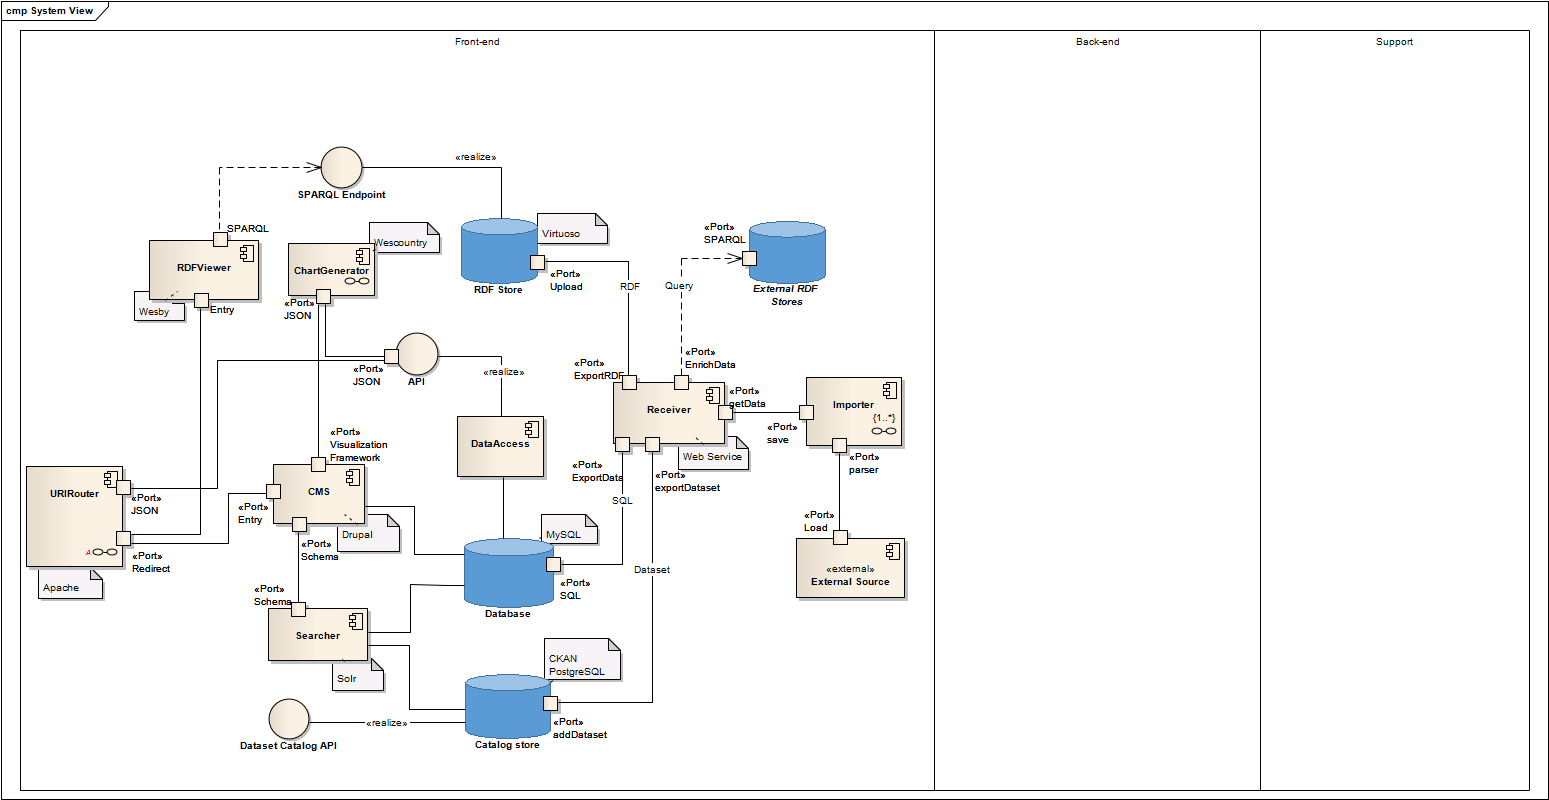
\includegraphics[height=\textwidth]{arquitectura/system_view}
		\caption{Diagrama de componentes del sistema}
		\label{fig:diagrama_componentes_sistema}
	\end{figure}
\end{landscape}


\subsubsection{Componentes}
Una vez mostrado el diagrama de componentes, se procederá a explicar el rol de cada uno de los componentes del sistema.  La descripción comenzará en los componentes más internos y terminará en los componentes más externos y cercanos al usuario del sistema.
\begin{description}
	\item[External source]  Las fuentes externas  serán fuentes de datos pertenecientes a organizaciones externas.  Estas fuentes proporcionan conjuntos de datos compuestos por indicadores y observaciones relativos a diferentes países y momentos del tiempo.  Como ya se ha mencionado en la sección ``\nameref{objetivos_proyecto}'' perteneciente al capítulo \ref{chapter01}, algunas de las fuentes externas con las que se trabajará son:
	\begin{itemize}
		\item el Banco Mundial (\textit{WorldBank})
		\item la Organización de las Naciones Unidas para la Alimentación y la Agricultura (\textit{FAO})
		\item la Organización Mundial de la Salud (\textit{WHO})
		\item el Instituto Internacional de Investigación sobre Políticas Alimentarias (\textit{IFPRI})
		\item la Organización para la Cooperación y el Desarrollo Económicos(\textit{OECD})
	\end{itemize}
	\item[Importer]  Los importadores  tendrán la tarea de transformar los conjuntos de datos provenientes de las fuentes externas a un formato común con el fin de unificar y asegurar un nivel de calidad mínimo para los datos que se insertarán en el portal.  Como se ha explicado en la sección ``\nameref{identificacion_actores}'' del capítulo \ref{chapter04}, los importadores serán los actores que interactuarán con el punto de entrada de datos, enviándole a este los conjuntos de datos ya procesados.
	\item[Receiver]  El Punto de Entrada de Datos  tendrá la misión de controlar todas las entradas de datos que se realicen hacia el portal.  Recibirá las peticiones de los importadores y almacenará los conjuntos de datos en varios servicios diferentes, concretamente: una base de datos SQL, una base de datos RDF y un catálogo de datos.  Además, el punto de entrada de datos también se encargará de enriquecer los datos antes de almacenarlos en el sistema, este enriquecimiento de datos tendrá lugar mediante la consulta de almacenamientos de RDF externos.  La arquitectura del punto de entrada de datos se verá con más detalle posteriormente en la sección ``\nameref{vista_receiver}'' de este mismo capítulo.
	\item[External RDF Stores]  Los almacenamientos (o \textit{endpoints}) de RDF externos son servicios externos que contienen información variada que se utilizará para enriquecer los datos que llegan al punto de entrada.  Un ejemplo de almacenamiento de RDF externo es \textit{DBPedia}\footnote{DBPedia contiene la información de la Wikipedia en forma de datos enlazados \url{http://dbpedia.org/About}}.
	\item[Database]  La base de datos será utilizada tanto por el gestor de contenidos y el framework de visualizaciones como por el API.  La base de datos será también uno de los lugares donde el punto de entrada almacene los catálogos de datos que llegan al portal.  El funcionamiento y esquema de la base de datos se detallará en la sección ``\nameref{diseno_modelo_datos}'' perteneciente a este mismo capítulo.
	\item[Catalog store - Dataset Catalog API]  El catálogo de datos será el encargado de almacenar los catálogos de datos que se utilizan en el portal acompañados de una serie de metadatos sobre su origen, creador, formato, etc.  Proveerá también una interfaz que permitirá a los usuarios navegar e incluso descargar en bruto los catálogos de datos almacenados en el sistema.  Como ya se explicó en la sección ``\nameref{chapter02:alternativas_seleccionadas}'' del capítulo \ref{chapter02}, el catálogo de datos seleccionado ha sido CKAN.  Al igual que la base de datos, el catálogo de datos será uno de los lugares en los que el punto de entrada almacena la información que llega al portal.
	\item[RDF Store - SPARQL endpoint]  El servidor semántico almacenará los datos en formato RDF y proveerá una punto de acceso SPARQL\footnote{SPARQL es un lenguaje de consultas capaz de manipular datos en formato RDF.  Para una mayor información al respecto véase \url{http://www.w3.org/TR/sparql11-overview/}} que podrá ser utilizado por los usuarios o por otros componentes del sistema.  Este componente será uno de los lugares donde el punto de entrada almacene los catálogos de datos que recibe.
	\item[API - DataAccess]  El API será el encargado de proporcionar una interfaz de acceso a los datos almacenados en la base de datos del sistema.  El API seguirá una arquitectura REST e incluirá un sistema de negociación de contenido con el que el cliente podrá seleccionar el formato en el que recibe los datos.  Algunos de los formatos soportados por el API serán JSON, CSV y XML.
	\item[Searcher]  El buscador será el encargado de indexar toda la información almacenada en el portal para proveer un sistema de búsqueda amigable a los usuarios.  Como se ha explicado en la sección ``\nameref{chapter02:alternativas_seleccionadas}'' del capítulo \ref{chapter02}, el buscador seleccionado ha sido Apache Solr.
	\item[CMS]  El gestor de contenidos tendrá una misión particularmente importante en el sistema final.  Será el componente que proveerá todos los subsistemas de la zona social (véase la sección ``\nameref{identificacion_subsistemas}''), además incluirá varios módulos que le permitirán comunicarse con otros componentes de la arquitectura.  Entre estos módulos destaca el módulo encargado de proporcionar el framework de soporte a las visualizaciones.  Los módulos que forman parte del gestor de contenidos podrán ser vistos con mayor detalle en la sección ``\nameref{vista_modulos_cms}'' de este mismo capítulo.
	\item[ChartGenerator]  Las visualizaciones serán las encargadas de transformar los datos en bruto almacenados en el sistema para presentarlos al usuario de una forma amigable y visual.  Par su construcción las visualizaciones utilizarán los datos devueltos por un framework que forma parte del subsistema de datos y que provee la información necesaria.  Las visualizaciones serán generadas por la librería \textit{Wescountry}
	\item[RDFViewer]  El visualizador de datos enlazados tendrá la misión de permitir a los usuarios navegar y visualizar los datos almacenados en el servidor semántico de una forma amigable y sin necesidad de realizar consultas SPARQL de forma manual.  Como se ha explicado en la sección ``\nameref{chapter02:alternativas_seleccionadas}'' del capítulo \ref{chapter02} el visualizador de datos enlazados seleccionado será \textit{Wesby}.
	\item[URIRouter]  El enrutador será el primer componente que entrará en acción del sistema ante las peticiones de los usuarios.  Su misión será redirigir la petición del usuario en función de su URL hacia el componente adecuado.  El enrutador utilizado será \textit{Apache}.
\end{description}
